

\documentclass{article}  
\bibliographystyle{unsrt}

\usepackage{bm}
\usepackage{graphicx}
\usepackage{subfigure}
\usepackage{amsmath}
\usepackage{esint}
\usepackage{soul}
\usepackage{listings}
\usepackage{xcolor}
\usepackage{tikz}
\usetikzlibrary{shapes, arrows}
\usetikzlibrary{positioning, shapes.geometric}

\title{Flowchart of coding for solute transport in DFNs}
\author         {Tingchang YIN\\Zhejiang University\\Westlake University}

%\date{\today}  
   

\tikzset{%
	bignode/.style     = {font=\fontsize{10}{10}\selectfont},
	mathnode/.style    = {execute at begin node=$,
		execute at end node=$},
	bigmathnode/.style = {bignode, mathnode}}

\begin{document}
	\maketitle
	\newpage
	\tableofcontents
	\newpage
\section{Flowchart}
The flow chart of coding for particle transport is below.
\begin{figure}[b]
	\centering
	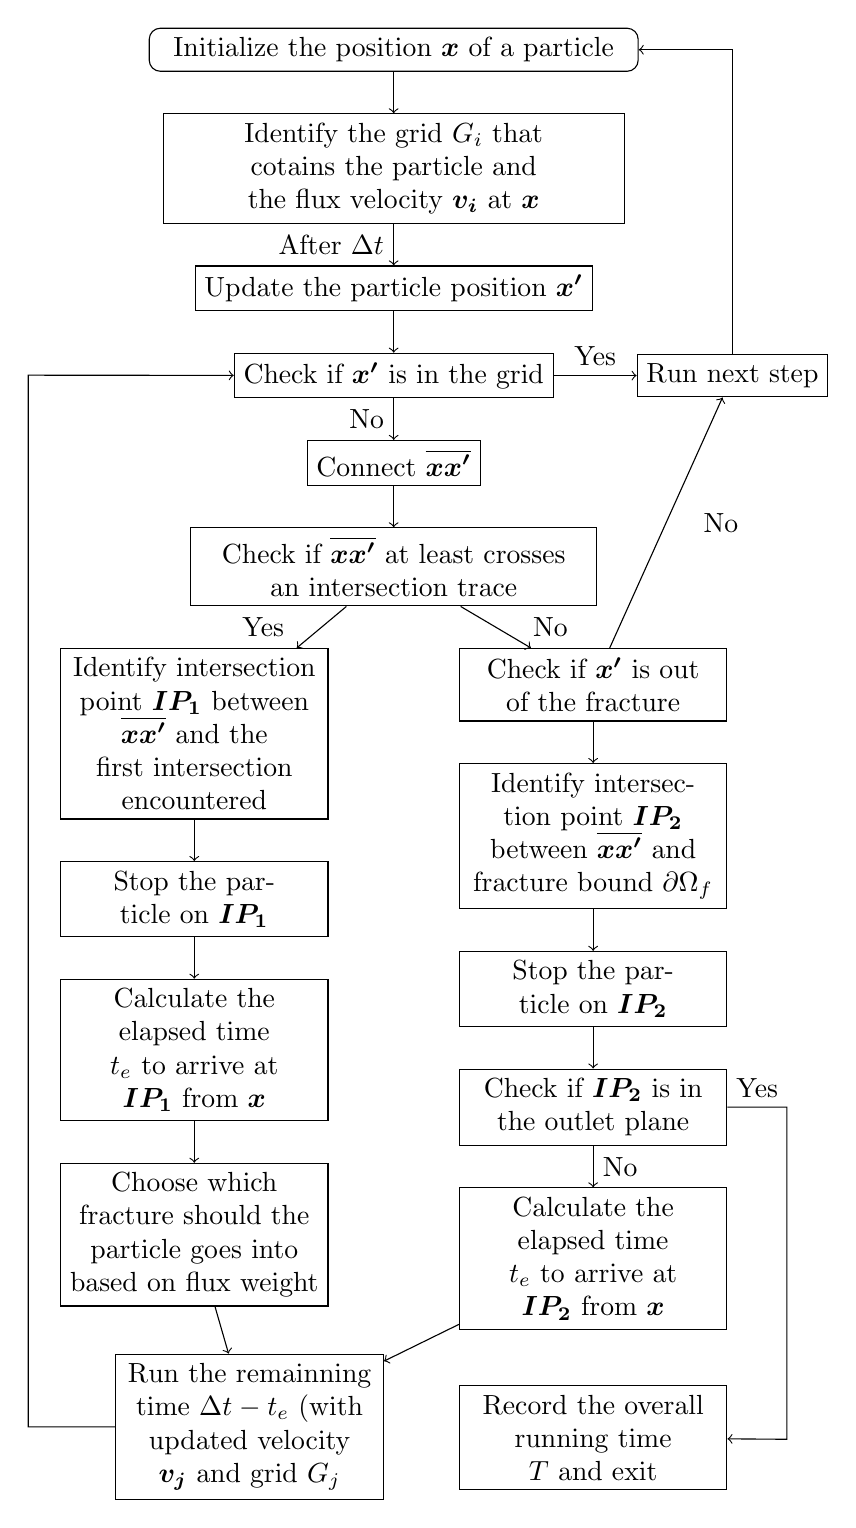
\begin{tikzpicture}[node distance=15pt]
		\node[draw, rounded corners, text width=170pt, align=center]                        (start)   {Initialize the position $\bm{x}$ of a particle};
		
		\node[draw, below=of start,  text width=160pt, align=center] (step x1) {Identify the grid $G_i$ that cotains the particle and the flux velocity $\bm{v_i}$ at $\bm{x}$};
		
		\node[draw, below=of step x1]                         (step 1)  {Update the particle position $\bm{x^\prime}$};
		\node [draw, below=of step 1] (step 2) {Check if $\bm{x^\prime}$ is in the grid};
		\node [draw, right=30pt of step 2] (step 3){Run next step};
		\node [draw, below=of step 2] (step 4){Connect $\bm{\overline{xx^\prime}}$};
		\node [draw, below=of step 4, text width=140pt, align=center] (step 5){Check if $\bm{\overline{xx^\prime}}$ at least crosses an intersection trace};
		
		\node [draw, below left= 15pt and -50pt of step 5, text width=90pt, align=center] (step 6) {Identify intersection point $\bm{IP_1}$ between $\bm{\overline{xx^\prime}}$ and the first intersection encountered};
		
		%---------
		\node [draw, below right= 15pt and -50pt of step 5, text width=90pt, align=center] (step 7) {Check if $\bm{x^\prime}$ is out of the fracture};
		\node [draw, below= of step 7, text width=90pt, align=center] (step 8) {Identify intersection point $\bm{IP_{2}}$ between $\bm{\overline{xx^\prime}}$ and fracture bound $\partial \Omega_f$};
		
		\node [draw, below=of step 8, text width=90pt, align=center] (step 9) {Stop the particle on $\bm{IP_{2}}$};
		\node [draw, below=of step 6, text width=90pt, align=center] (step 10) {Stop the particle on $\bm{IP_{1}}$};
		\node [draw, below=of step 10, text width=90pt, align=center] (step 11) {Calculate the elapsed time $t_e$ to arrive at $\bm{IP_{1}}$ from $\bm{x}$};
		\node [draw, below=of step 11, text width=90pt, align=center] (step 12) {Choose which fracture should the particle goes into based on flux weight};
		
		\node [draw, below left=270pt and -70pt of step 5, text width=90pt, align=center] (step 13) {Run the remainning time $\Delta t - t_e$ (with updated velocity $\bm{v_j}$ and grid $G_j$};	
		
		\node [draw, below=of step 9, text width=90pt, align=center] (step 15) {Check if $\bm{IP_{2}}$ is in the outlet plane};
		
		\node [draw, below=of step 15, text width=90pt, align=center] (step 14) {Calculate the elapsed time $t_e$ to arrive at $\bm{IP_{2}}$ from $\bm{x}$};
		
		\node [draw, below=20pt of step 14, text width=90pt, align=center] (step 16) {Record the overall running time $T$ and exit};
		
		\draw[->] (step 6)--(step 10);
		\draw[->] (step 10)--(step 11);
		\draw[->] (step 11)--(step 12);
		\draw[->] (step 12)--(step 13);
		\draw[->] (step 14)--(step 13);
		\draw[->] (step 7)--(step 8);
		\draw[->] (step 8)--(step 9);
		\draw[->] (step 9)--(step 15);
		\draw[->] (step 15)--node[right] {No}(step 14);
		
		\draw[->] (start)--(step x1);
		\draw[->] (step x1)--node[left] {After $\Delta t$} (step 1);
		\draw[->] (step 1)--(step 2);
		\draw[->] (step 2)--node[above] {Yes} (step 3);
		\draw[->] (step 3)--(step 3|-start)->(start);
		\draw[->] (step 2)--node[left] {No} (step 4);
		\draw[->] (step 4)--(step 5);
		\draw[->] (step 5)--node[left=10pt] {Yes} (step 6);
		\draw[->] (step 5)--node[right=10pt] {No} (step 7);
		\draw[->] (step 7)--node[right=10pt] {No} (step 3);
		% \draw[->] (step 13)--(step 15)--(step 15|-step 2)->(step 2);
		\draw[->] (step 13)--+(-80pt, 0)--+(-80pt, 380pt)->(step 2);
		\draw[->] (step 15)--node[above] {Yes}+(70pt, 0)--+(70pt,-120pt)--(step 16);	
	\end{tikzpicture}
\end{figure}

\end{document}